\documentclass[12pt]{article}
\usepackage[a4paper, total={7.5in, 11in}]{geometry}
%\usepackage{array}
\usepackage{graphicx, subfig, wrapfig, fancyhdr, lastpage, multicol ,color,arydshln,makecell, tcolorbox, mhchem,chemfig}
\newcommand\headerMe[2]{\noindent{}#1\hfill#2}
\usepackage[mathscr]{euscript}
\usepackage{tabularray}

\setlength{\columnseprule}{1pt}
\def\columnseprulecolor{\color{blue}}


\pagestyle{fancy}
\fancyhf{}

\cfoot{ \vspace{-0.8cm}\em{Page \thepage \hspace{1pt} / \pageref{LastPage}}}
\begin{document}

\headerMe{Royaume du Maroc}{année scolaire \emph{2022-2023}}\\
\headerMe{Ministère de l'Éducation nationale, }{  }\\
\headerMe{du Préscolaire et des Sports}{Établissement : \emph{Lycée SKHOR qualifiant}}\\
%\vspace{-1cm}
\begin{center}
%Devoir Surveillé  N°1 \\
	Examen National blanc\\
    2ème année baccalauréat Sciences physiques\\
%Durée 2h00
    \vspace{.2cm}
\hrulefill
\Large{--Chimie(7 points)--}
\hrulefill\\

    \emph{Les  parties sont indépendantes}
    %\emph{Les deux parties sont indépendantes}
\end{center}
%end Headerss------------------------
%__________________Chimie ______________________-
%%%%%%%+_+_+_+_+_+_+_+_+_Partie1

 \section*{Partie 1 : Durée de fonctionnement d'une pile\dotfill (3 POINTS)  }
\begin{wrapfigure}{r}{0.3\textwidth}
	\vspace{-1.2cm}
\begin{center}
	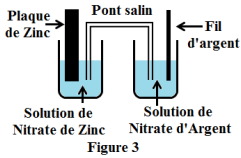
\includegraphics[width=0.3\textwidth]{./img/chimie1.png}
\end{center}
\end{wrapfigure}

 \emph{ \textbf{ Une pile est conçue pour alimenter des circuits électriques, elle met en jeu des transformations
chimiques afin de récupérer de l'énergie électrique.
Cette partie a pour but de déterminer la durée de fonctionnement d'une pile.
}}

On réalise la pile zinc-argent schématisée sur la figure (3). On relie les électrodes de la
pile à un conducteur ohmique en série avec un ampèremètre et on observe le passage d’un
courant électrique dans le circuit extérieur de la pile.

\textbf{Données :}
\begin{itemize}

	\item Couples mis en jeu: $Zn^{2+}_{(aq)}/Zn_{(s)}$ ; $Ag^+_{(aq)}/Ag_{(s)}$
	\item Les deux solutions ont même concentration molaire $C_0=0,20mol.L^{-1}$ et même volume $V_0 =100mL$ .
	\item La masse initiale de l’électrode de zinc est  $m_0(Zn) = 2,0g$.
	\item $1F =96500 C.mol^{-1}$ ; $M(Zn) = 65,4 g.mol^{-1}$.
	\item La constante d’équilibre associée à l’équation $\ce{Zn_{(s)} + 2Ag^+_{(aq)} <=>[1][2] Zn_{(aq)}^{2+} +2Ag_{(s)}}$ est \textbf{K = $10^{52}$}
\end{itemize}

\begin{tabular}{c|l}
0,75	& \makecell[l]{\textbf{1. }Calculer la valeur du quotient de la réaction $Q_{r,i}$ à l’état initial du système chimique.\\Prévoir le sens d’évolution spontané de ce système.  }\\ 

	1 & \makecell[l]{\textbf{2. }En déduire les polarités des électrodes. Justifier votre réponse. }\\
	0,25 & \makecell[l]{\textbf{3. }Déterminer le réactif limitant.}\\
	1 & \makecell[l]{\textbf{4. }La pile débite un courant continu d’intensité constante $I = 0,15 A$ et s'épuise après\\
	une longue durée $\Delta{t}$ . Calculer la valeur de $\Delta{t}$. }\\
\end{tabular}

 \section*{Partie 2 : Synthèse d’un ester\dotfill (4 POINTS)  }
 Un chimiste se propose de synthétiser un ester à odeur de banae (\textbf{l'acétate d'iso-amyle})   utilisé pour parfumer certaines confiseries.

 Pour cela, il introduit dans un ballon, en prenant les précautions nécessaires :

 \begin{itemize}
	 \item un Volume $V_A = 8,6mL$ d'acide éthanoique (de formule chimique $C_2H_4O_2$ et de densité par rapport à l'eau d=1,05).
	 \item un Volume $V_B =13,8mL$ de l'alcool iso-amylique de formule $C_5H_12O$ (soit 0,15mol).
	 %\item $\chemfig{CH_3-C(=[::+60]O)(-[::-60]O-CH_2-CH_2-C(-[2]CH_3)-CH_3}$
	 \item (\textbf{l'acétate d'iso-amyle})  $\chemfig{CH_3-C(=[::+60]O)(-[::-60]O-CH_2-CH_2-CH(-[2]CH_3)-CH_3)}$

 \end{itemize}

 On donne  : $M(H)=1g/mol$ ; $M(C)=12g/mol$ ; $M(O)=16g/mol$ et $\rho_{eau} = 1g/mol$

\begin{tabular}{c|l}
0,75	& \makecell[l]{\textbf{1. }Montrer que le mélange initial (acide + alcool) est équimolaire.}\\ 

		& \makecell[l]{\textbf{2. }La réaction de synthèse est schématisée comme suit: \\acide éthanoique + alcool \ce{<=>} ester +eau . }\\
	0,5 & \makecell[l]{\textbf{2.a. }Citer les trois principales propriétés de cette réaction.}\\
	0,5 & \makecell[l]{\textbf{2.b. }Dresser le tableau d'avancement décrivant l'évolution du système au cours du temps.}\\


	1 & \makecell[l]{\textbf{2.c. }Déterminer la quantité maximale d'acétate d'iso-amyle que peut synthétiser ce chimiste \\sachant que la constante d'équilibre de la réaction de synthèse de l'ester est égale à 4.}\\

	0,75 & \makecell[l]{\textbf{3. }Afin d'améliorer le rendement de cette réaction, le chimiste pense aux opérations suivantes: \\
		\textbf{ - ajouter un catalyseur : l'acide sulfurique concentré par exemple}\\
	\textbf{- réaliser une distillation fractionnée consistant à éliminer progressivement} l'eau formée.
Parmi ces deux propositions , choisir en justifiant celle qui vous semble raisonnable.}\\


		0,5 & \makecell[l]{\textbf{3. } Le chimiste a réaliser une autre expérience en remplaçant l'acide éthanoique par son \\anhydride. Ecrire l'équation de la réaction qui se produit.}\\
\end{tabular}


\begin{center}
%Devoir Surveillé  N°1 \\
%Durée 2h00
    %\vspace{.2cm}
\hrulefill
\Large{--Physique (13 points)--}
\hrulefill\\

    \emph{Les  parties sont indépendantes}
    %\emph{Les deux parties sont indépendantes}
\end{center}


 \section*{Partie 1: Application des ondes ultrasonores\dotfill (2,5 POINTS)  }

 \begin{tcolorbox}
 \emph{Actuellement certaines voitures sont équipées de plusieurs capteurs tels que les capteurs ultrasons
et les capteurs LASER. Ces capteurs servent à faciliter le contrôle de son environnement proche
qui peut atteindre une distance de 2m.}

\emph{Le tableau de bord de ces nouvelles gammes de voitures est très développé, il est constitué d'un
ensemble d'indicateurs et de témoins qui renseignent le conducteur sur le fonctionnement du
moteur et sur les paramètres de conduite (vitesse instantanée, température extérieure ...). Certains
circuits électroniques du tableau de bord comportent des condensateurs, des bobines ... Le confort
dans ces voitures est assuré par plusieurs éléments et accessoires parmi lesquels, les amortisseurs
qui utilisent des ressorts.}
\end{tcolorbox}


\begin{wrapfigure}{r}{0.25\textwidth}
  \begin{center}
	  \vspace{-1cm}
	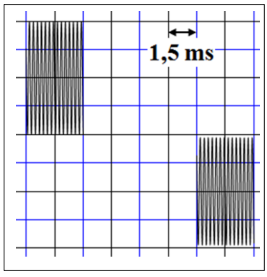
\includegraphics[width=0.25\textwidth]{./img/ondes01.png}
  \end{center}
\end{wrapfigure}

Une voiture est équipée d’un système comportant un émetteur (E) et un récepteur (R) d’ultrasons
placés côte à côte à l’arrière du véhicule.

Lors d'un stationnement, l'émetteur (E) envoie des ultrasons sous forme de salves. Ces ultrasons sont
captés par le récepteur (R) après réflexion sur un obstacle situé à la distance d de (E).

\textbf{Données : }Vitesse de propagation des ultrasons dans l’air : $v_0$=$340 m.s^{-1}$.

\begin{tabular}{c|l}
	1  & \makecell[l]{\textbf{1. }Répondre par vrai ou faux aux propositions a, b, c et d suivantes: }\\
\end{tabular}

\begin{center}
	\begin{tabular}{|c|l|}
 a & L'onde ultrasonore est une onde longitudinale \\
 b & L'onde ultrasonore se propage dans le vide \\  
 c & La propagation des ultrasons se fait avec transport de matière \\
 d & La fréquence des ultrasons varie en changeant le milieu de propagation \\  
\end{tabular}
\end{center}


\begin{tabular}{c|l}
	& \makecell[l]{\textbf{2. }L'oscillogramme ci-contre donne le signal émis par l'émetteur (E)
et le signal réfléchi par \\le récepteur (R).
 }\\ 

	0,5 & \makecell[l]{\textbf{2.1. }Déterminer graphiquement la durée $\tau$ entre le signal émis et le signal reçu.
 }\\
	0,75 & \makecell[l]{\textbf{2.2. }Calculer la distance d qui sépare l’obstacle de l'émetteur (E). }\\
	0,25 & \makecell[l]{\textbf{2.3. }On considère un point M du milieu de propagation qui se	trouve à la distance $EM = \frac{d}{2}$ \\de l'émetteur (E).Recopier sur votre copie le numéro de la question et écrire la lettre
\\correspondante à la proposition vraie :L'élongation $y_M(t)$ de M en fonction de l'élongation de \\l'émetteur (E) est: }\\
\end{tabular}


\begin{center}
	\begin{tabular}{|c|c|}
		
a & $y_M(t) = y_E(t-\tau)$ \\
b & $y_M(t) = y_E(t-\frac{\tau}{2})$ \\
c & $y_M(t) = y_E(t - \frac{\tau}{4})$ \\
d & $y_M(t) = y_E(t-2.\tau)$ \\ 
\end{tabular}
\end{center}

%\hrulefill
%\Large{Physique 13pts/78min}
%\hrulefill\\
\section*{Partie 2 :Étude de la cible de berkélium 249\dotfill(1,5pts)}

\begin{tcolorbox}
La  première  étape  de  la  synthèse  de  l’élément  117  a  consisté  en  la  fabrication  du berkélium : un mélange de curium et d’américium a été irradié durant 250 jours par un intense  flux  de  neutrons  [...].  Il  a  fallu  ensuite 90  jours  pour  séparer  et  purifier  les  22 milligrammes de berkélium produits. [...] Ce précieux élément, déposé sur un film de titane, [...] a été soumis, 150 jours durant, au flux de calcium. " Il fallait faire vite, selon Hervé  Savajols,  chercheur  au  Grand  Accélérateur  national  d’ions  lourds  (GANIL),  car l’isotope du berkélium utilisé ayant une période de 320 jours, à la fin de l’expérience, il ne restait que 70\% du berkélium initial ".
\end{tcolorbox}


\begin{tabular}{c|l}
	0,25  & \makecell[l]{\textbf{1. }On  donne  l’équation  incomplète  de  la  désintégration  du  noyau  de  berkélium 249 :\\ $^{249}_{97}Bk \rightarrow ^{249}_{98}Cf + ......$ \\En précisant les lois de conservation utilisées, identifier la particule émise.  De quel type de \\radioactivité s’agit-il ici ?  }\\

		0,25 & \makecell[l]{\textbf{2. }Sachant  que  le  bombardement  de  la  cible  de  berkélium  a  duré  150 jours,  vérifier  l’affirmation  :\\ "   À  la  fin  de  l’expérience,  il  ne  restait  que 70\% du berkélium initial "}\\
	& \makecell[l]{\textbf{3. }Activité de la source de berkélium de masse égale à 22 mg :  }\\

		0,5 & \makecell[l]{\textbf{3.1 }Déterminer  le  nombre  initial  $N_0$  de  noyaux  de  berkélium  249  dans l’échantillon  produit  \\sachant  que  la  masse  d’un  atome  de  berkélium 249 est $m_{atome} = 4,136.10^{-25}Kg$.  }\\
		0,5 & \makecell[l]{\textbf{3.2 }Exprimer  l’activité  initiale  $a_0$  de  l’échantillon  de  berkélium  249  en fonction de $N_0$ et $t_{1/2}$. \\La calculer en becquerel.}\\

\end{tabular}

\section*{Partie 3 :Application des ondes ultrasonores \dotfill(5pts)}

\emph{Beaucoup d’appareils électriques contiennent des circuits qui se composent de condensateurs, de
bobines, de conducteurs ohmiques ...La fonction de ces composantes varie selon leurs domaines
d’utilisation et la façon dont elles sont montées dans les circuits.}

Cet partie a pour objectifs :
\begin{itemize}
	\item de vérifier les caractéristiques d’une bobine (b) et de l’utiliser dans un circuit RLC série.
	\item  d’étudier la modulation d’amplitude.
\end{itemize}


\textbf{\underline{I- Détermination des caractéristiques d’une bobine.}}

On réalise le montage expérimental représenté sur la figure 1 comprenant :
\begin{itemize}
	\item  Une bobine (b) d’inductance L et de résistance r.
	\item  Un conducteur ohmique (D) de résistance R.
	\item  Un générateur de tension (G) de force électromotrice E.
	\item  Un ampèremètre (A) de résistance négligeable.
	\item  Un interrupteur K.
\end{itemize}

A l’instant t = 0, on ferme l’interrupteur K , et on visualise à l’aide d’un oscilloscope à mémoire les
variations de la tension $u_{PQ}(t)$ entre les pôles du générateur (G) et de la tension $u_R(t)$ entre les bornes du conducteur ohmique (D). On obtient les courbes 1 et 2 représentées sur la figure 2.


\begin{center}
  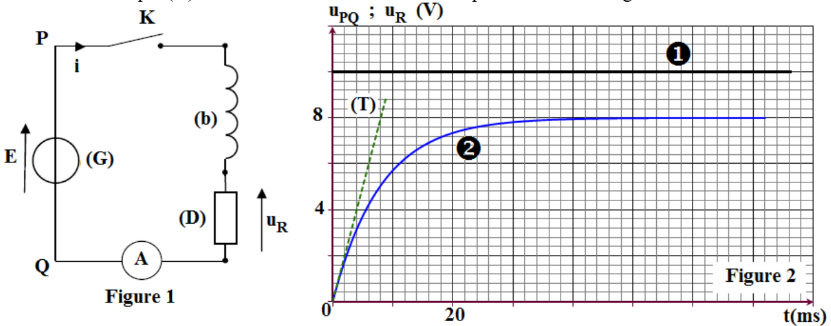
\includegraphics[width=0.8\textwidth]{./img/Rl01.png}
\end{center}



La droite (T) représente la tangente à la courbe 2 à l’instant t=0 .
Dans le régime permanent, l’ampèremètre (A) indique la valeur I = 0,2A.

\begin{tabular}{c|l}
	0,5  & \makecell[l]{\textbf{1. }Montrer que l’équation différentielle que vérifie la tension $u_R$ s’écrit sous la forme \\: $L.\frac{du_R}{dt} + (R+r).u_R - E.R = 0$}\\
	0,5 & \makecell[l]{\textbf{2. }Sachant que la solution de l’équation différentielle s’écrit sous la forme : $u_R = U_0.(1-e^{-\frac{t}{\tau}})$,\\trouver l’expression des constantes $U_0$ et $\tau$ en fonction des paramètres du circuit.}\\
		0,75 & \makecell[l]{\textbf{3. }Trouver l’expression de la résistance r de la bobine (b) en fonction de E , I et $U_0$. Calculer \\la valeur
de r.}\\
			0,5 & \makecell[l]{\textbf{4. }Déterminer graphiquement la valeur numérique de t et vérifier que la valeur de l’inductance \\L de la
bobine est $L=0,4H$}\\
		\end{tabular}




\textbf{\underline{II- Etude du dipôle RLC}}

On réalise le montage représenté sur la figure 3 qui comprend une bobine (b), le générateur (G) de force électromotrice E, un condensateur de capacité C, un conducteur ohmique de résistance $R' = 10 \Omega$ et un interrupteur K.

Après avoir chargé totalement le condensateur, on bascule l’interrupteur K à la position 2 à l’instant $t = 0$ et on visualise à l’aide d’un oscilloscope à mémoire les variations de la tension $u_c$ aux bornes du
condensateur en fonction du temps .On obtient l’oscillogramme représenté sur la figure 4.

\begin{center}
  \includegraphics[width=0.8\textwidth]{./img/rlc_01.png}
\end{center}

\begin{tabular}{c|l}
	0,25  & \makecell[l]{\textbf{1. }Donner le nom du régime associé à la courbe de la figure 4. }\\
	0,25 & \makecell[l]{\textbf{2. }Déterminer graphiquement la pseudo-période T.}\\
	0,5 & \makecell[l]{\textbf{3. }On suppose que la pseudo-période est égale à la période propre T0 de l’oscillateur électrique.
\\Déduire la valeur de la capacité C du condensateur }\\
\\
		\end{tabular}


\textbf{\underline{III - Etude de la modulation d’amplitude}}

Afin d’obtenir un signal modulé en amplitude, on utilise
un circuit intégré multiplieur $X$ (fig.6).
On applique à l’entrée :

- $E_1$: la tension $u_1(t) = s(t) + U_0$ avec $s(t) = S_m.cos(2.\pi.f_s.t)$représentant le signal informatif et $U_0$ une composante
continue de la tension. 

- $E_2$: une tension sinusoïdale représentant la porteuse $u_2 = U_m.cos(2.\pi.F_p.t)$

- La tension de sortie $u_s(t)$ obtenue est  $u_s(t) = k.u_1(t).u_2(t)$.

- k est une constante qui dépend du circuit intégré X.
- Rappel: $2cos(a).cos(b) = cos(a+b) + cos(a-b)$

\begin{tabular}{c|l}
	1  & \makecell[l]{\textbf{1. }Montrer que us(t) s’écrit sous la forme : \\$u_s(t) = \frac{A.m}{2}.cos(2.\pi.f_1.t) + A.cos(2.\pi.f_2.t) + \frac{A.m}{2}.cos(2.\pi.f_3.t)$ , où m est le taux de modulation\\ et A une constante.}\\
	0,75 & \makecell[l]{\textbf{2. }La figure 7 représente le spectre de fréquences formé de trois raies de la tension modulée us(t). \\Déterminer m et
la fréquence fs. La modulation est-elle bonne ?}\\
		\end{tabular}


\begin{center}
  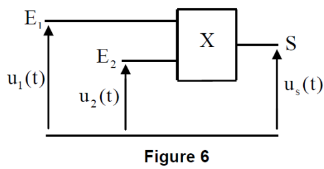
\includegraphics[width=0.3\textwidth]{./img/mod01.png}
  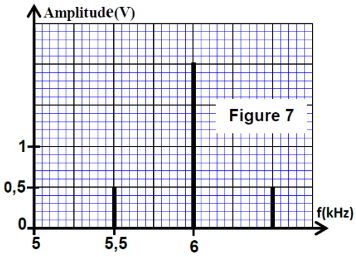
\includegraphics[width=0.3\textwidth]{./img/mod02.png}
\end{center}






\section*{Partie 4 :Etude du mouvement d’un pendule pesant \dotfill(2,75pts)}

\begin{wrapfigure}{r}{0.16\textwidth}
	\vspace{-1.2cm}
\begin{center}
  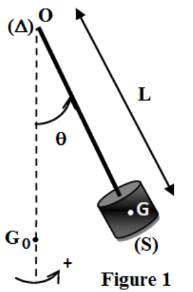
\includegraphics[width=0.16\textwidth]{./img/pendule011.png}
\end{center}
\end{wrapfigure}

Un pendule pesant, de centre d’inertie G et de masse m, constitué d’une tige et d’un corps solide (S).
Ce pendule peut effectuer un mouvement de rotation autour d’un axe horizontal ( D) fixe passant par l’extrémité O de la tige (figure 1 ).
On désigne par $J_{\Delta}$  le moment d’inertie du pendule pesant par rapport à l’axe $(\Delta)$ et par L la distance
séparant G de l’axe ($\Delta$).

\textbf{Données : }

\begin{itemize}
	\item $g \approx 10 m.s^{-2}$ ; $m = 400g$ ; $L=50cm$.
	\item Pour les oscillations de faible amplitude on prendra : $sin(\theta) \approx \theta$ et $1-cos(\theta) \approx \frac{\theta^2}{2}$ avec $\theta $ en radian.
	\item $\pi^2 \approx 10$
\end{itemize}

On écarte le pendule de sa position d’équilibre stable, dans le sens positif,
d’un angle $\theta_m$ très petit, puis on le lâche sans vitesse initiale à l’instant $t=0$.

A chaque instant, la position du pendule est repérée par son abscisse
angulaire $\theta$. On néglige les frottements et on travaille dans l’approximation
de faibles oscillations
\begin{center}
\textbf{Etude dynamique}
\end{center}
\begin{tabular}{c|l}
	0,5  & \makecell[l]{\textbf{1. }Trouver en appliquant la relation fondamentale de la dynamique, l’équation différentielle du
\\mouvement du pendule pesant. }\\
		0,5  & \makecell[l]{\textbf{2. }Trouver l’expression de la période propre $T_0$ de ce pendule en fonction de m , g , L et $J_{\Delta}$ pour \\que
		la solution de l’équation différentielle s’écrit sous la forme $\theta(t) = \theta_m.cos(\frac{2.\pi}{T_0}.t + \phi)$. }\\
	0,25  & \makecell[l]{\textbf{3. }Vérifier par une analyse dimensionnelle que l’expression de $T_0$ a la dimension du temps.}\\

	0,5  & \makecell[l]{\textbf{4. }Sachant que la valeur de la période propre est $T_0 \approx 0,7s$ . Calculer $J_{\Delta}$ }\\
	\end{tabular}
\begin{center}
\textbf{Etude énergétique}
\end{center}
On choisit le plan horizontal passant par le point $G_0$, position de G à l’équilibre stable, comme état de
référence de l’énergie potentielle de pesanteur $E_{pp}(\theta = 0) = 0$.

La figure 2 représente le diagramme d’énergie du pendule étudié.


\begin{center}
  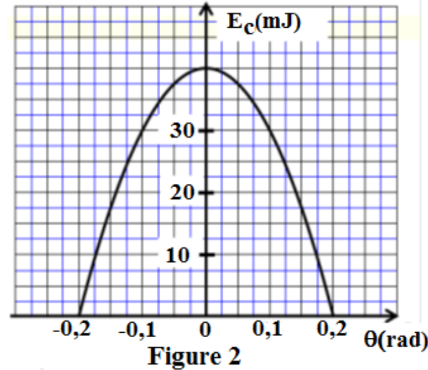
\includegraphics[width=0.35\textwidth]{./img/pendule_pesa.png}
\end{center}





\begin{tabular}{c|l}
	  & \makecell[l]{\textbf{1. }Déterminer la valeur de :}\\
		0,25  & \makecell[l]{\textbf{1.1. }L'abscisse angulaire maximale $\theta_m$}\\
	0,25  & \makecell[l]{\textbf{1.2. }L’énergie mécanique $E_m$ du pendule.}\\

	0,5  & \makecell[l]{\textbf{2. }Calculer les deux abscisses angulaires $\theta_1$ et $\theta_2$ pour lesquelles l’énergie potentielle est égale
\\l’énergie cinétique. } \\
	\end{tabular}




\section*{Partie 5: Test d'amortissement d'une voiture \dotfill(1,25pts)  }

\begin{wrapfigure}{r}{0.24\textwidth}
	\vspace{-1.4cm}
\begin{center}
  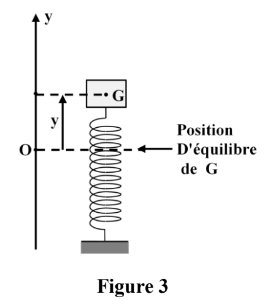
\includegraphics[width=0.24\textwidth]{./img/pendule22.png}
\end{center}
\end{wrapfigure}


Pour les voitures, le système d'amortissement permet d'atténuer les oscillations verticales se produisant sur la route. Ce système se compose au niveau
de chaque roue d'un ressort et d'un amortisseur
(généralement à huile).

On modélise la voiture par un solide (S)
de masse m et de centre d'inertie G
qui repose sur un ressort vertical de constante de raideur K (figure 3).

Pour étudier le système oscillant $({solide (S) +  ressort})$, on
 repère les positions de G
par son ordonnée y sur un axe
vertical $Oy$ orienté vers le haut. L'origine O est choisi à la
position d'équilibre de G.


\begin{tabular}{c|l}
	
	 0,5 & \makecell[l]{\textbf{1. }Recopier sur votre copie le numéro de la question et écrire la lettre \\correspondante à \\la proposition vraie:
		 L'expression de la période propre $T_0$ des oscillations libres du système \\oscillant est:\\ a:$T_0 = 2\pi.\frac{K}{m}$ \hspace{1cm} b:$T_0 = 2\pi.\sqrt{\frac{K}{m}}$ \hspace{1cm} c:$T_0 = 2\pi.\sqrt{\frac{m}{K}}$ \hspace{1cm} d:$T_0 = 2\pi.\sqrt{K.m}$ 
 \\Justifier la réponse par analyse dimensionnelle.}\\

	  & \makecell[l]{\textbf{2. }Lors d'un test du système d'amortissement de deux voitures $(V_1)$ et $(V_2 )$, On a relevé les \\variations $y(t)$ des positions du centre d'inertie G de chaque voiture. Ces variations sont \\indiquées sur la figure (4) pour les deux voitures.}\\


	 0,5 & \makecell[l]{\textbf{2.1 }On considère que la pseudo période T est égale à la période propre $T_0$ de l'oscillateur. \\Calculer la valeur de la raideur K , sachant que $ m=1300 kg$ (on prendra $\pi^2 \approx 10 $).}\\

 0,25 & \makecell[l]{\textbf{2.2 }Indiquer, en justifiant la réponse, la voiture qui présente plus de confort.}\\
\end{tabular}

\begin{center}
  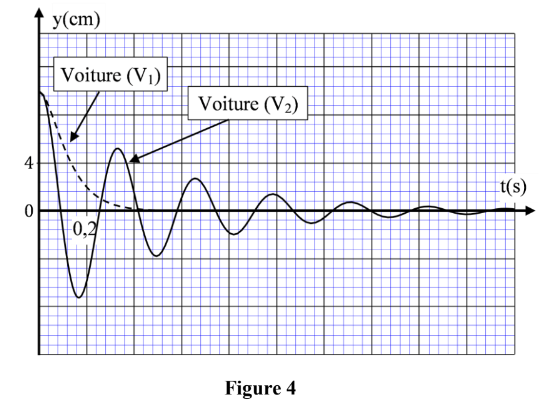
\includegraphics[width=0.48\textwidth]{./img/oscillo.png}
\end{center}

\end{document}
